% \documentclass[8pt,aspectratio=1610]{beamer}
\documentclass{beamer}
\usepackage[orientation=landscape, size=a2, scale=1.75]{beamerposter}
% \beamertemplateshadingbackground{brown!70}{yellow!10}
\mode<presentation>
{
  %\usetheme{Warsaw}
  \usecolortheme{crane}
  % or ...

  \setbeamercovered{transparent}
%    \setbeamercovered{invisible}
  % or whatever (possibly just delete it)
}
% \setbeamertemplate{navigation symbols}{}
% \setbeamertemplate{footline}[frame number]{}
\usepackage{tikz,pgfplots}
\pgfplotsset{compat=newest}
\usepackage[utf8]{inputenc}
\usetikzlibrary{patterns}
\usepackage{amssymb}
\usepackage{amsmath}
\usepackage{colortbl}
%\usepackage{multicol}
\usepackage{cancel}
\usepackage{ulem}
\usepackage{multirow}
\usepackage{relsize}
\usepackage{algorithm}
\usepackage{algorithmic}
\usepackage{forloop}% http://ctan.org/pkg/forloop
\newcounter{loopcntr}
\usepackage{tkz-euclide}
\usetkzobj{all}
\newcommand{\rpt}[2][1]{%
  \forloop{loopcntr}{0}{\value{loopcntr}<#1}{#2}%
}
%\pagestyle{plain}
%\input{defs2}
\def\opt{{\textsc{OPT}_k}}
\def\const{{\mathrm{const}}}
\def\nnz{{\mathrm{nnz}}}
\def\r{\sfrac{\sigma_{\w}^2}{\sigma_{\xib}^2}}
\def\rm{\sfrac{\sigma_{\xib}^2}{\sigma_{\w}^2}}
\def\cmark{\Green{\checkmark}}
\def\xmark{\Red{\large\sffamily x}}
\newcommand{\pdet}{{\mathrm{pdet}}}
\newcommand{\MSPE}[1] {{\mathrm{MSPE}\big[#1\big]}}
\newcommand{\MSE}[1] {{\mathrm{MSE}\big[#1\big]}}
\def\Poisson{{\operatorname{Poisson}}}
\def\PB{{\operatorname{PB}}}
\newcommand{\DP}[1]{\mathcal{DP}^{#1}}
\def\Ic{\mathcal{I}}
\def\Jc{\mathcal{J}}
\def\Mc{\mathcal M}
\def\Ec{\mathcal E}
\def\sr{{\mathrm{sr}}}
\def\ktd{{k^{\underline{d}}}}
\def\Det{{\mathrm{Det}}}
\def\detu{{\widecheck{\mathrm{Det}}_\mu^\gamma}}
\def\deto{{\widehat{\mathrm{Det}}_\mu^\gamma}}
\def\Zu{{\widecheck{Z}_\mu^{\gamma}}}
\def\Zo{{\widehat{Z}_\mu^{\gamma}}}
\def\Zun{{\widecheck{Z}_\mu^{\gamma_n}}}
\def\Zon{{\widehat{Z}_\mu^{\gamma_n}}}
\newcommand{\Er}{\mathrm{Er}}
\newif\ifDRAFT
\DRAFTtrue
\ifDRAFT
\newcommand{\marrow}{\marginpar[\hfill$\longrightarrow$]{$\longleftarrow$}}
\newcommand{\niceremark}[3]
   {\textcolor{red}{\textsc{#1 #2:} \marrow\textsf{#3}}}
\newcommand{\ken}[2][says]{\niceremark{Ken}{#1}{#2}}
\newcommand{\manfred}[2][says]{\niceremark{Manfred}{#1}{#2}}
\newcommand{\michael}[2][says]{\niceremark{Michael}{#1}{#2}}
\newcommand{\michal}[2][says]{\niceremark{Michal}{#1}{#2}}
\newcommand{\feynman}[2][says]{\niceremark{Feynman}{#1}{#2}}
%\usepackage[inline]{showlabels}
\else
\newcommand{\ken}[1]{}
\newcommand{\michael}[1]{}
\newcommand{\michal}[1]{}
\newcommand{\feynman}[1]{}
\fi
\newcommand{\norm}[1]{{\| #1 \|}}

\newcommand{\deff}{d_{\textnormal{eff}}}
\def\ee{\mathrm{e}}
\newcommand\mydots{\makebox[1em][c]{.\hfil.\hfil.}}
\def\Sd{\mathscr{S}_{\!d}}
\newcommand{\dx}{\dxy_{\!\cal X}}
\newcommand{\dxk}{\dxy_{\!\cal X}^k}
\newcommand{\dk}{\dxy^k}
\newcommand{\dxy}{\mathrm{D}}
\def\simiid{\overset{\textnormal{\fontsize{6}{6}\selectfont
i.i.d.}}{\sim}}
%\newcommand{\Dxy}{D_{\!\cal X\!,\cal Y}}
\def\vskx{{\mathrm{VS}_{\!\dx}^k}}
\def\vsk{{\mathrm{VS}_{\!D}^k}}
\def\vskxm{{\mathrm{VS}_{\!\dx}^{k-1}}}
\def\vskm{{\mathrm{VS}_{\!D}^{k-1}}}
\def\vsdx{{\mathrm{VS}_{\!\dx}^d}}
\def\vsd{{\mathrm{VS}_{\!D}^d}}
\newcommand{\vs}[1]{{\mathrm{VS}_{\!D}^{#1}}}
\newcommand{\sigd}{\boldsymbol\Sigma_{\!\dx}}
\def\wols{\w_{\mathrm{LS}}}
\def\wds{\boldsymbol\w_{\!D}^*}
\def\kd{K_{\!\dx}}

\def\poly{{\mathrm{poly}}}
\def\polylog{{\mathrm{polylog}}}
\def\DPP{{\mathrm{DPP}}}
\def\DPPcor{{\DPP_{\!\mathrm{cor}}}}
\def\DPPens{{\DPP_{\!\mathrm{ens}}}}
\newcommand{\DPPreg}[1]{{\DPP_{\!\mathrm{reg}}^{#1}}}
\def\Vol{{\mathrm{VS}}}
\def\Lev{{\mathrm{Lev}}}
\newcommand\todod[1]{\Red{\# DH: #1}}
\newcommand{\explain}[2]{\mathrel{\overset{\makebox[0pt]{\text{\tiny
#1}}}{#2}}}
\def\tot {{\mathrm{tot}}}
\def\checkmark{\tikz\fill[scale=0.4](0,.35) -- (.25,0) --
(1,.7) -- (.25,.15) -- cycle;}
\newcommand{\mnote}[1]{{\bf\large \Magenta{*}}\marginpar{\small \Magenta{#1}}}
\newcommand{\bnote}[1]{{\bf #1}}

\newcommand{\sqrtshort}[1]{{\sqrt{\white{\Big|}\!\!\smash{\text{\fontsize{9}{9}\selectfont$#1$}}}}}
\newenvironment{proofof}[2]{\par\vspace{2mm}\noindent\textbf{Proof of {#1} {#2}}\ }{\hfill\BlackBox}
\newcommand{\sets}[2]
{{\hspace{-0.3mm}[\hspace{-0.3mm}#1\hspace{-0.3mm}]\hspace{-0.3mm}\choose
\hspace{-0.3mm}#2\hspace{-0.3mm}}}
\DeclareMathOperator{\sgn}{\textnormal{sgn}}
\DeclareMathOperator{\adj}{\textnormal{adj}}
\def\Rb{{\mathbf{R}}}
\DeclareMathOperator{\ws}{\widetilde{\w}}
\newcommand{\inote}[1]{{\bf {#1}}}
\def\xib{\boldsymbol\xi}
\def\Sigmab{\mathbf{\Sigma}}
\def\Sigmabh{\widehat{\Sigmab}}
\def\Sigmabt{\widetilde{\Sigmab}}
\def\S{\mathbf{S}}
\def\T{\mathbf{T}}
\def\xt{\tilde{x}}
\def\xbt{\widetilde{\x}}
\def\xbh{\widehat{\x}}
\def\ubh{\widehat{\u}}
\def\dom {{\mathrm{dom}}}
\def\val {{\mathrm{val}}}
\def\out {{\mathrm{out}}}
\def\iin  {{\mathrm{iin}}}
\def\s {\mathbf{s}}
\def\q {\mathbf{q}}
\def\qt{\tilde{q}}
\def\itld {j}
\def\ubt {\tilde{\u}}
\def\n{\{1..n\}}
\def\cb {\mathbf{c}}
\def\cW{\mathcal W}
\def\Xt{\widetilde{X}}
\def\Dbt{\widetilde{\D}}
\def\xtb{\tilde{\mathbf{x}}}
\def\ytb{\tilde{\mathbf{y}}}
\def\Xtb{\widetilde{\mathbf{X}}}
\def\Xbb{\overline{\X}}
\def\Xb{{\bar{\X}}}
\def\ybb{\overline{\y}}
\def\f{{\mathbf{f}}}
\def\g{{\mathbf{g}}}
\def\fbb{{\overline{\f}}}
\def\fb{{\overline{f}}}
\def\Xc{\mathcal{X}}
\def\W{\mathbf W}
\def\L{\mathbf{L}}
\def\Rb{\mathbf R}
\def\Pc{\mathcal{P}}
\def\Nc{\mathcal{N}}
\def\Pt{\widetilde{P}}
\def\Hc{\mathcal{H}}
\def\Wc{\mathcal{W}}
\def\Cc{\mathcal{C}}
\def\p{\mathbf p}
%\def\r{\mathbf r}
\def\Y{\mathbf Y}
\def\H{\mathbf H}
\def\K{\mathbf K}
\def\Kh{\widehat{K}}
\def\Kbh{{\widehat{\K}}}
\def\Q{\mathbf Q}
\def\Qbar{{\bar{\mathbf Q}}}
\def\Ytb{\widetilde{\mathbf{Y}}}
\def\c{{n-d\choose s-d}}
\DeclareMathOperator{\Proj}{Proj}
\newcommand{\Span}{\mathrm{span}}
\newcommand{\ofsubt}[1]{\mbox{\scriptsize \raisebox{0.25pt}{$(#1)$}}}
%\raisebox{0.5pt}{$($}}#1\mbox{\tiny \raisebox{0.5pt}{$)$}}}
\newcommand{\ofsub}[1]{\mbox{\small \raisebox{0.0pt}{$(#1)$}}}
%\newcommand{\ofsubb}[1]{\mbox{\footnotesize \raisebox{0.5pt}{$(#1)$}}}
%\newcommand{\ofsub}[1]{(#1)}
%\newcommand{\ofsub}[1]{\mbox{\tiny$|$\hspace{-0.5pt}\raisebox{-0.5pt}{$#1$}}}
\newcommand{\of}[2]{{#1{\!\ofsub{#2}}}}
\newcommand{\oft}[2]{{#1{\!\ofsubt{#2}}}}
\newcommand{\fof}[2]{{#1({#2})}}
\newcommand{\yof}[2]{{#1{\ofsub{#2}}}}
%\newcommand{\yofb}[2]{{#1{\ofsubb{#2}}}}
\newcommand{\lazy}{FastRegVol}
\newcommand{\volsamp}{RegVol}

\newcommand{\Sm}{{S_{-i}}}
\newcommand{\Sp}{{S_{+i}}}
\ifx\BlackBox\undefined
\newcommand{\BlackBox}{\rule{1.5ex}{1.5ex}}  % end of proof
\fi
%\renewcommand{\dagger}{+}
\DeclareMathOperator*{\argmin}{\mathop{\mathrm{argmin}}}
\DeclareMathOperator*{\argmax}{\mathop{\mathrm{argmax}}}
\DeclareMathOperator*{\diag}{\mathop{\mathrm{diag}}}
\def\x{\mathbf x}
\def\y{\mathbf y}
\def\ybh{\widehat{\mathbf y}}
\def\ybb{\bar{\mathbf y}}
\def\xbb{\bar{\mathbf x}}
\def\yb{{\bar y}}
\def\ybt{\widetilde{\mathbf y}}
\def\yh{\widehat{y}}
\def\yhb{\widehat{\y}}
\def\yt{\widetilde{y}}
\def\z{\mathbf z}
\def\a{\mathbf a}
\def\b{\mathbf b}
\def\w{\mathbf w}
\def\v{\mathbf v}
\def\m{\mathbf m}
\def\wbh{\widehat{\mathbf w}}
\def\wh{\widehat{\mathbf w}}
\def\vbh{\widehat{\mathbf v}}
\def\wbt{\widetilde{\mathbf w}}
\def\e{\mathbf e}
\def\zero{\mathbf 0}
\def\one{\mathbf 1}
\def\u{\mathbf u}
\def\ubbar{\bar{\mathbf u}}
\def\f{\mathbf f}
\def\ellb{\boldsymbol\ell}

\def\X{\mathbf X}
\def\Xs{\widetilde{\X}}
\def\B{\mathbf B}
\def\A{\mathbf A}
\def\C{\mathbf C}
\def\U{\mathbf U}
\def\Ubt{\widetilde{\mathbf U}}
\def\Ubh{\widehat{\mathbf U}}
\def\Ubbar{\bar{\mathbf U}}
\def\F{\mathbf F}
\def\D{\mathbf D}
\def\V{\mathbf V}
\def\M{\mathbf M}
\def\Mh{\widehat{\mathbf M}}
%\def\S{\mathbf S}
\def\Stb{\widetilde{\mathbf{S}}}
\def\Sbh{\widehat{\mathbf{S}}}
\def\St{\widetilde{\S}}
\def\Sh{\widehat{S}}
\def\Sc{\mathcal{S}}
\def\Fc{\mathcal{F}}
\def\Vc{\mathcal{V}}
\def\Bc{\mathcal{B}}
\def\Dc{\mathcal{D}}
\def\Z{\mathbf Z}
\def\Zbh{\widehat{\mathbf Z}}
\def\Zbt{\widetilde{\mathbf Z}}
\def\Abh{\widehat{\mathbf A}}
\def\I{\mathbf I}
\def\Ic{\mathcal I}
\def\II{\mathbf {I \!\,I}}
%\def\II{\boldsymbol {\mathbb I}}
\def\A{\mathbf A}
\def\P{\mathbf P}
\def\Ph{\widehat{\mathbf P}}
\def\cP{\mathcal P}
\def\cR{\mathcal R}
\def\Xt{\widetilde{\mathbf{X}}}
\def\Xh{\widehat{\mathbf{X}}}
\def\Rh{\widehat{R}}
\def\Ot{\widetilde{O}}
\def\At{\widetilde{\A}}


\def\E{\mathbb E}
\def\R{\mathbb R}
\def\N{\mathbb N}
\def\Pr{\mathrm{Pr}}
%\def\C{\mathbb C}
\def\tr{\mathrm{tr}}
\def\Sbar{{\bar{S}}}
\def\cS{{\mathcal{S}}}
\def\Tbar{{\bar{T}}}
\def\Tt{{\widetilde{T}}}
\def\rank{\mathrm{rank}}
\def\Prob{\mathrm{Prob}}
\def\Var{\mathrm{Var}}
\def\Xinv{(\X^\top\X)^{-1}}
\def\XinvS{(\X_S\X_S^\top)^{-1}}
\def\ABinvS{(\A_S\B_S^\top)^{-1}}
\def\ABinv{(\A\B^\top)^{-1}}
\def\xinv{\x_i^\top\Xinv\x_i}
\def\Xinvr{(\lambda\I+\X_{-1}^\top\X_{-1})^{-1}}
\def\pdet{\mathrm{pdet}}
\newcommand{\vol}{\mathrm{vol}}
%\newcommand{\defeq}{:=}
\newcommand{\defeq}{\stackrel{\textit{\tiny{def}}}{=}}
\newcommand{\di}{{[d+1]_{-i}}}
\newcommand{\cov}{\mathrm{cov}}
\let\origtop\top
\renewcommand\top{{\scriptscriptstyle{\origtop}}} % this makes transpose not so big

\definecolor{silver}{cmyk}{0,0,0,0.3}
\definecolor{yellow}{cmyk}{0,0,0.9,0.0}
\definecolor{reddishyellow}{cmyk}{0,0.22,1.0,0.0}
\definecolor{black}{cmyk}{0,0,0.0,1.0}
\definecolor{darkYellow}{cmyk}{0.2,0.4,1.0,0}
\definecolor{orange}{cmyk}{0.0,0.7,0.9,0}
\definecolor{darkSilver}{cmyk}{0,0,0,0.1}
\definecolor{grey}{cmyk}{0,0,0,0.5}
\definecolor{darkgreen}{cmyk}{0.6,0,0.8,0}
\newcommand{\Red}[1]{{\color{red}  {#1}}}
\newcommand{\Purple}[1]{{\color{purple}  {#1}}}
\newcommand{\Magenta}[1]{{\color{magenta}{#1}}}
\newcommand{\Green}[1]{{\color{darkgreen}  {#1}}}
\newcommand{\Blue}[1]{\color{blue}{#1}\color{black}}
\newcommand{\Orange}[1]{\textcolor{orange}{#1}\color{black}}
\newcommand{\Brown}[1]{{\color{brown}{#1}\color{black}}}
\newcommand{\Grey}[1]{{\color{grey}{#1}\color{black}}}
\newcommand{\white}[1]{{\textcolor{white}{#1}}}
\newcommand{\yellow}[1]{{\textcolor{reddishyellow}{#1}}}
\newcommand{\darkYellow}[1]{{\textcolor{darkYellow}{#1}}}
\newcommand{\grey}[1]{{\textcolor{grey}{#1}}}

\DeclareMathOperator{\half}{\frac{1}{2}}

\ifx\proof\undefined
\newenvironment{proof}{\par\noindent{\bf Proof\ }}{\hfill\BlackBox\\[2mm]}
\fi

\ifx\theorem\undefined
\newtheorem{theorem}{Theorem}
\fi

\ifx\example\undefined
\newtheorem{example}{Example}
\fi

\ifx\condition\undefined
\newtheorem{condition}{Condition}
\fi
\ifx\property\undefined
\newtheorem{property}{Property}
\fi

\ifx\lemma\undefined
\newtheorem{lemma}{Lemma}
\fi

\ifx\proposition\undefined
\newtheorem{proposition}{Proposition}
\fi

\ifx\remark\undefined
\newtheorem{remark}{Remark}
\fi

\ifx\corollary\undefined
\newtheorem{corollary}{Corollary}
\fi

\ifx\definition\undefined
\newtheorem{definition}{Definition}
\fi

\ifx\conjecture\undefined
\newtheorem{conjecture}{Conjecture}
\fi

\ifx\axiom\undefined
\newtheorem{axiom}{Axiom}
\fi

\ifx\claim\undefined
\newtheorem{claim}{Claim}
\fi

\ifx\assumption\undefined
\newtheorem{assumption}{Assumption}
\fi

\ifx\condition\undefined
\newtheorem{condition}{Condition}
\fi


\edef\polishl{\l}
\setlength{\columnsep}{0.7em}
\setlength{\columnseprule}{0mm}
\setlength{\arrayrulewidth}{1pt} 

\newcommand{\svr}[1]{{\textcolor{darkSilver}{#1}}}
\definecolor{brightyellow}{cmyk}{0,0,0.7,0.0}
\definecolor{lightyellow}{cmyk}{0,0,0.3,0.0}
\definecolor{lighteryellow}{cmyk}{0,0,0.1,0.0}
\definecolor{lightestyellow}{cmyk}{0,0,0.05,0.0}

%  \fboxsep=3pt
% %\fboxsep=0mm%padding thickness
% \fboxrule=2pt%border thickness


\setkeys{Gin}{width=0.7\textwidth}

% \title{Unbiased estimates for linear regression\\
% via volume sampling}
% \author[]{Micha{\polishl } Derezi\'{n}ski and Manfred Warmuth}

\begin{document}

\begin{frame}
  \frametitle{
    \centering\textrm{\textbf{\LARGE Improved guarantees
        and a multiple-descent curve}}\\
\centering\textrm{\textbf{\LARGE
  for Column Subset Selection and the Nystr\"om method}}\\[-2mm]
\textit{\large Micha{\polishl } Derezi\'{n}ski, \ Rajiv Khanna,
  \ Michael Mahoney\qquad UC Berkeley}\\[-5mm]
}
\begin{columns}
  \begin{column}{0.32\textwidth}

  \begin{block}{Interpretable dimensionality reduction}

  \underline{Example application}: \textit{Genetics}
  \begin{center}
    \includegraphics[width=\textwidth]{figs/snp.png}
  \end{center}


  \begin{itemize}
  \item \cite{paschou2007pca} (in \textit{PLOS Genetics}, 2007) \\[-1mm]
{\scriptsize\textit{``PCA-correlated SNPs for structure
    identification in worldwide human populations''}}
  \item  \cite{mahoney2009cur} (in \textit{Proc.~of the NAS}, 2009)\\[-1mm]
    \hspace{-5mm}{\scriptsize\textit{``CUR matrix decompositions for
        improved data analysis''}}
  \end{itemize}
\end{block}
    
 \begin{block}{Subset selection}
    \begin{columns}
    \begin{column}{.43\textwidth}
      \begin{center}
        \emph{Column Subset Selection} \\[1mm]
\begin{tikzpicture}[scale=.9]
  \draw (0,0) rectangle (8,4);
  \draw (5,.75) node {\small Data matrix $\A$};
    \draw[fill=blue!20] (1,0) rectangle (2.5,4);
    %\draw (-1,2) node {\mbox{$\A\ =$}};
    %\draw (6.5,2) node {\mbox{$\in\R^{m\times n}$}};
    \draw [decorate,decoration={brace}] (1,4.1) -- (2.5,4.1);
    \draw (1.75,4.6) node {\small $S$}; 
  \end{tikzpicture}
\end{center}
\vspace{6mm}

{\small
\begin{enumerate}
\item Feature selection
\item Dimensionality reduction
\item Interpretability
\end{enumerate}}
\end{column}
\begin{column}{.53\textwidth}
  \begin{center}
    \emph{Nystr\"om method}\\[1mm]
\begin{tikzpicture}[scale=1]
  \draw (0,0) rectangle (5,5);
  \draw (2.5,.75) node {\small Kernel matrix $\K$};
    \draw[fill=blue!20] (1,2.5) rectangle (2.5,4);      
    %\draw (-1,2) node {\mbox{$\K\ =$}};
    %\draw (6.5,2) node {\mbox{$\in\R^{n\times n}$}};
    \draw [decorate,decoration={brace}] (1,5.1) -- (2.5,5.1);
    \draw (1.75,5.6) node {\small $S$};
    \draw [decorate,decoration={brace}] (-.1,2.5) -- (-.1,4);
    \draw (-.55,3.25) node {\small $S$}; 
  \end{tikzpicture}  
\end{center}
{\small
\begin{enumerate}
\item Kernel machines
\item Gaussian Process regression
\item Independent Component Analysis
\end{enumerate}}
\end{column}
\end{columns}
\end{block}

 \begin{block}{Interpretable low-rank approximation}
  \begin{columns}
    \begin{column}{0.5\textwidth}
      \begin{align*}
        \Er = \big\|\A - \mathrm{Proj}(\A)\big\|_F^2
      \end{align*}
      \emph{Optimal choice}:\\
      {\small Top $k$ \textit{principal components}}\\
      \Red{\small Not interpretable!}\\[1mm]
      
      \emph{Goal}:\\
      {\small Find best \textit{interpretable} choice}
    \end{column}
    \begin{column}{0.45\textwidth}
      \begin{center}

        \begin{tikzpicture}[scale=1]

        \draw (-3.2,-3.2) -- (3.2,3.2);
        \tkzDefPoint(0,1){A};         \tkzDefPoint(0.5,.5){A1}; \tkzDrawSegment[thick,red](A,A1);
        \tkzDefPoint(1.8,.5){B};     \tkzDefPoint(1.15,1.15){B1}; \tkzDrawSegment[thick,red](B,B1);
        \tkzDefPoint(2.5,1.5){C};   \tkzDefPoint(2,2){C1}; \tkzDrawSegment[thick,red](C,C1);
        \tkzDefPoint(-1.5,-.3){D}; \tkzDefPoint(-.9,-.9){D1}; \tkzDrawSegment[thick,red](D,D1);
        \tkzDefPoint(-2,-.3){E};    \tkzDefPoint(-1.15,-1.15){E1}; \tkzDrawSegment[thick,red](E,E1);
        \tkzDefPoint(1,1.5){F};  \tkzDefPoint(1.25,1.25){F1}; \tkzDrawSegment[thick,red](F,F1);
        \tkzDefPoint(.5,-.5){G};  \tkzDefPoint(0,0){G1}; \tkzDrawSegment[thick,red](G,G1);
        \tkzDefPoint(2,4.4/1.65){H};  \tkzDefPoint((2+4.4/1.65)/2,(2+4.4/1.65)/2){H1}; \tkzDrawSegment[thick,red](H,H1);
        \tkzDefPoint(-1,0){I};  \tkzDefPoint(-.5,-.5){I1}; \tkzDrawSegment[thick,red](I,I1);
        \tkzDefPoint(1.1,2.5){J};  \tkzDefPoint(1.8,1.8){J1}; \tkzDrawSegment[thick,red](J,J1);
        \tkzDefPoint(-1.32,-1.76){K};  \tkzDefPoint(-1.54,-1.54){K1}; \tkzDrawSegment[thick,red](K,K1);
        \tkzDefPoint(-1.5,-2.5){L};  \tkzDefPoint(-2,-2){L1}; \tkzDrawSegment[thick,red](L,L1);


            \draw [thick,blue] (-3.3/1.4,-4.4/1.4) -- (3.3/1.4,4.4/1.4);
            % \tkzDrawSegment[thick,red](H,K);
            \foreach \n in {H,K} \node at (\n)[circle,fill=cyan,inner
            sep=2.25pt]{};


        \foreach \n in {A,B,C,D,E,F,G,H,I,J,K,L} \node at (\n)[circle,fill=blue,inner
        sep=1.5pt]{};
        \foreach \n in {A1,B1,C1,D1,E1,F1,G1,H1,I1,J1,K1,L1} \node at (\n)[circle,fill=black,inner
        sep=1pt]{};        

      \end{tikzpicture}   
    \end{center}
  \end{column}
\end{columns}
\vspace{5mm}

\underline{Cost of Interpretability}:\\[-11mm]

\begin{align*}
  \text{Approximation factor}\quad=\quad
  \frac{\Er(\text{best subset $S$ of size $k$})}{\Er(\text{top $k$
  principal components})}
\end{align*}

\end{block}

  \end{column}


  \begin{column}{0.32\textwidth}

    
    \begin{block}{Multiple-descent curve}
        \begin{align*}
\text{\underline{Prior work}~\cite{pca-volume-sampling}:}\quad
    \underbrace{\text{Approximation
    factor}\quad
\leq\quad k+1}_{\text{worst-case optimal!}} %\qquad\text{for size $k$}
  \end{align*}
  We go beyond worst case analysis!\vspace{2mm}
  
    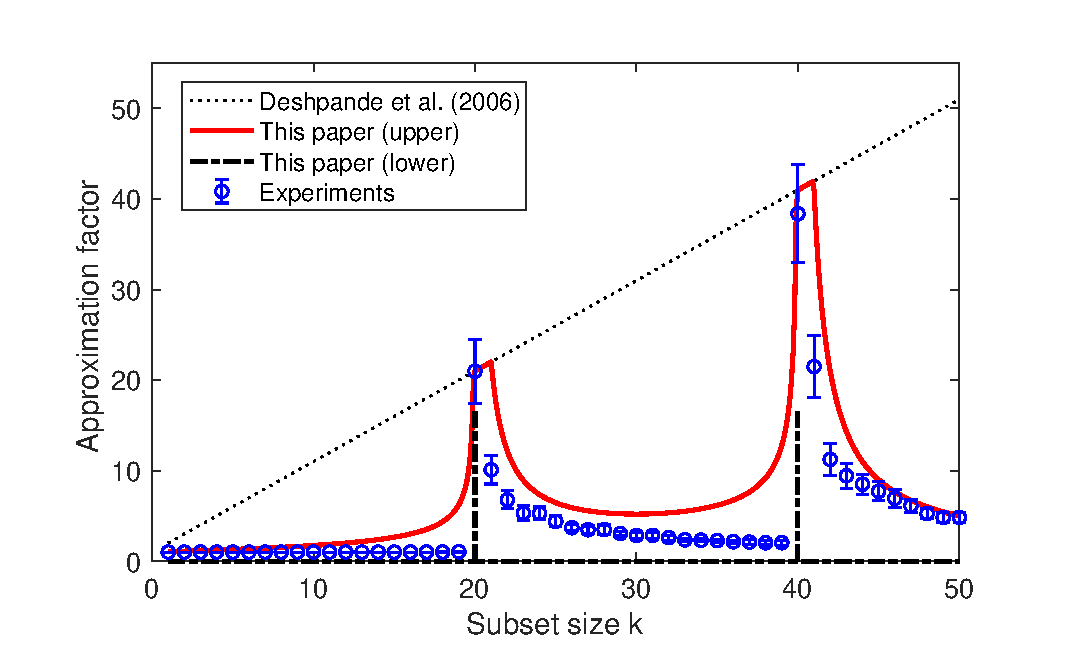
\includegraphics[width=\textwidth]{../figs/nystrom/nystrom-bounds}

    \vspace{-4mm}    
    \begin{align*}
      \text{sharp spectral drop}\ &\Longrightarrow\ \text{large spike}\\[2mm]
      \text{smooth spectral decay}\ &\Longrightarrow\ \text{no spikes}
    \end{align*}

    
  \end{block}

  
  \begin{block}{Connection to double descent}
  \emph{Double descent}: Exhibited by generalization error \cite{BHMM19}
  \vspace{1cm}
  
  \begin{columns}
    \begin{column}{.6\textwidth}
      ``Classical'' ML: \hfill\textit{parameters} $\ll$ \textit{data}\\
    ``Modern'' ML: \hfill \textit{parameters} $\gg$ \textit{data}
\end{column}
\begin{column}{.35\textwidth}
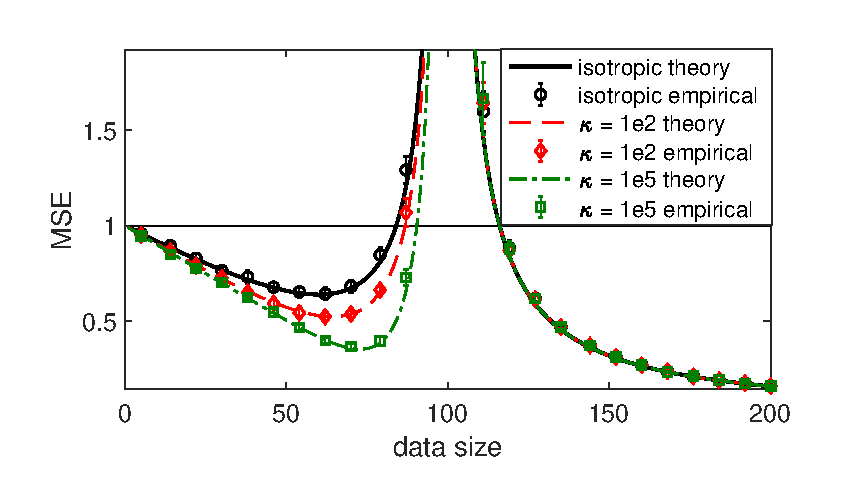
\includegraphics[width=\textwidth]{figs/descent-intro-nice}
\end{column}
\end{columns}
\vspace{1cm}

\emph{Connections}:
\begin{enumerate}
\item Correlated with the condition number of the data \cite{double-descent-condition}
\item Multiple peaks are possible
  \cite{liang2020multiple,BLLT19_TR}
\item  Similar techniques can be used for the analysis \cite{surrogate-design}\\[-1mm]
{  \footnotesize\textit{``Exact expressions for
    double descent...''}, NeurIPS'20.}
\end{enumerate}
\vspace{5mm}
  
\end{block}



\end{column}


\begin{column}{.32\textwidth}


\begin{block}{Improved guarantees under smooth spectral decay}
Smooth spectral decay \ $\Longrightarrow$ \ no spikes!
\vspace{5mm}

\begin{enumerate}
\item 
  \emph{Polynomial decay}:\quad $i$th singular
  value \ $\asymp\ i^{-p}$
  \vspace{-2mm}
  \begin{align*}
    \text{Approximation factor}\ \leq\ O(1+p)\quad\text{for all $k$}
  \end{align*}
  \vspace{0mm}
  
\item 
  \emph{Exponential decay}:\ $i$th singular
    value \ $\asymp\ (1-\delta)^i$
    \vspace{-2mm}
    \begin{align*}
    \text{Approximation factor}\ \leq\ O(1+\delta k)\quad\text{for all $k$}
    \end{align*}
\end{enumerate}
\end{block}

  \begin{block}{\underline{Method}: Determinantal Point Processes (DPPs)}
  \emph{Non-i.i.d.}~randomized selection of column subset $S$\\[2mm]

  \emph{Negative correlation}: $\Pr(i\in S\mid j\in S) < \Pr(i\in S)$
  \vspace{-2mm}
  
\begin{center}
  \includegraphics[width=0.6\textwidth]{../figs/gue.png}
  \vspace{-3mm}
  
  \small  i.i.d.~(left) versus DPP (right)%
\end{center}
\vspace{-2mm}
\begin{itemize}
\item \emph{Fast algorithms}: \cite{alpha-dpp} (NeurIPS'20)\\[-1mm]
  {\footnotesize\textit{``Sampling
      from a $k$-DPP without looking at all items''}}
  \item \emph{Learn more}: \cite{dpps-in-randnla}
    (Notices of the AMS)\\[-1mm]
    {\footnotesize\textit{``Determinantal point processes in randomized numerical
      linear algebra''}}
\end{itemize}
%\let\thefootnote\relax\footnotetext{Image from \cite{dpp-ml}}  
\end{block}


  \begin{block}{Multiple-descent in real-world subset selection}
  \emph{Kernel}: Gaussian RBF,
  $\langle\a_i,\a_j\rangle_\text{K}=\exp(-\|\a_i\!-\!\a_j\|^2/\sigma^2)$\\[3mm]
  
  \centering
  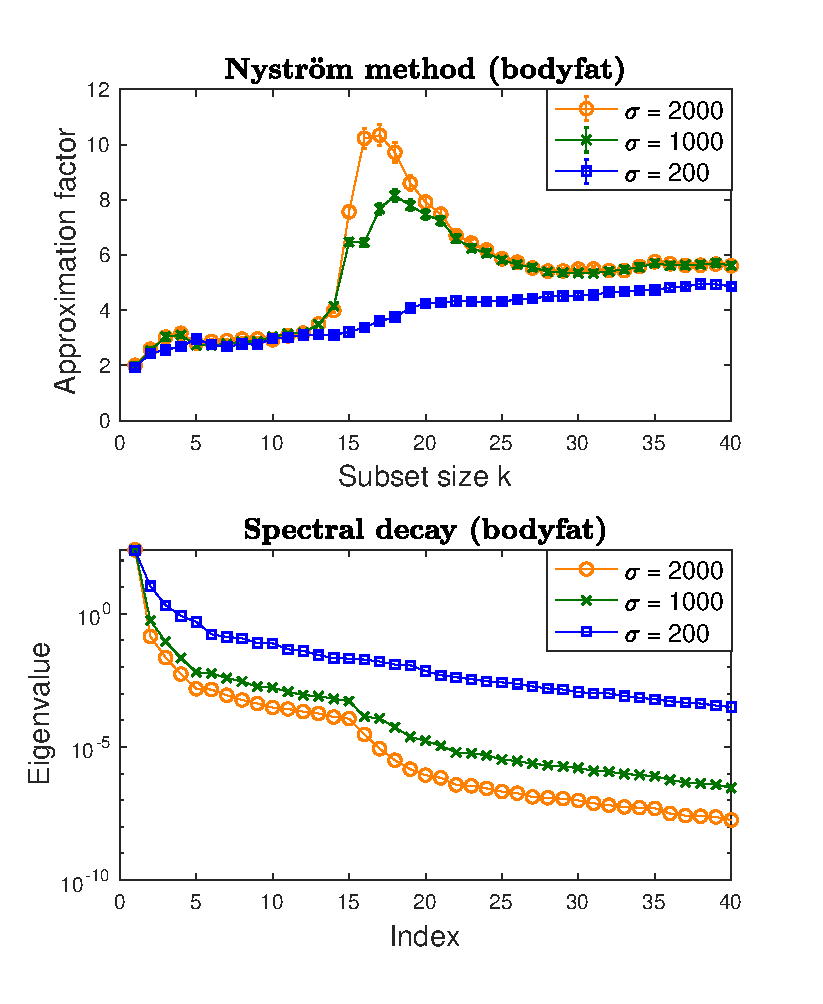
\includegraphics[width=0.45\textwidth]{../figs/nystrom/rbf-bodyfat-double}
  \hspace{5mm}
  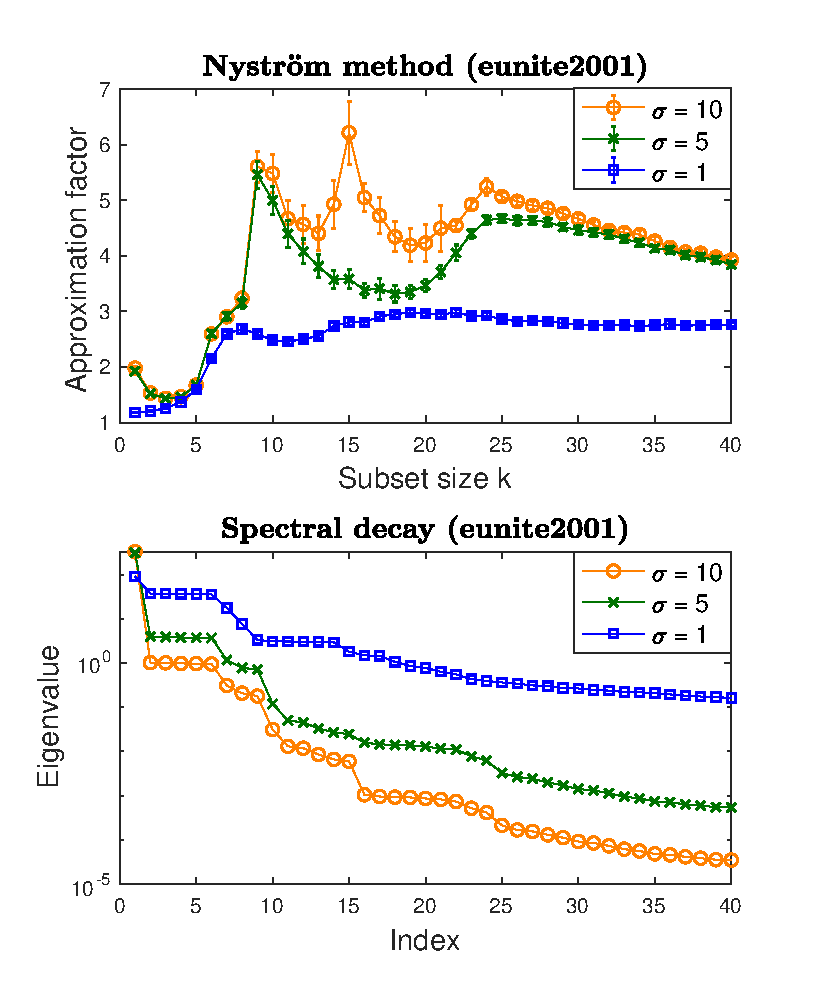
\includegraphics[width=0.45\textwidth]{../figs/nystrom/rbf-eunite2001-double}
  
  % \let\thefootnote\relax\footnotetext{Datasets from the Libsvm repository \cite{libsvm}}  
\end{block}

\end{column}
\end{columns}
\vspace{1cm}

\bibliographystyle{alpha}
  \bibliography{../pap}

\end{frame}


\end{document}
